\section{Installing libraries}
Install requests.
\begin{verbatim}[autogobble]
    > pip install requests
\end{verbatim}

%%%%%%%%%%%%%%%%%%%%%%%%%%%%%%%%%%%%%%%%%%%%%%%%%%%%%%
\section{Introduction}
\begin{itemize}
    \item We will be using the website: \url{http://quotes.toscrape.com/} which is a website used specifically to webscrap. 
    \item It consists of quotes and tags which you can try to scape.
\end{itemize}

\subsection{Webscrapping}
\begin{itemize}
    \item First lets import the required libraries:
        \begin{minted}[autogobble]{py}
            import requests
            from bs4 import BeautifulSoup
        \end{minted}
    
    \item The requests object will provide all the information that the website responded. HTML, status code, etcetera.
        \begin{minted}[autogobble]{py}
            website = requests.get('http://quotes.toscrape.com/')
            print(website)
            # <Response [200]>
        \end{minted}
    
    \item The .text attribute in the website gives us the html response. We can use this to send the html string to parse to beautifyl soup. The html string from the site and the type of parser we are going to use must be speficied in the BeautifulSoup object constructor.
        \begin{minted}[autogobble]{py}
            website = requests.get('http://quotes.toscrape.com/')
            soup = BeautifulSoup(website.text, 'html.parser')
        \end{minted}
    
    \item Now we can start to extract elements form this web string.
        \begin{minted}[autogobble]{py}
            title = soup.find('title')
            print(title)
            # <title>Quotes to Scrape</title>
            print(title.text)
            # Quotes to Scrape
        \end{minted}
    
    \item To get the first link on the website:
        \begin{minted}[autogobble]{py}
            print(soup.find('a'))
            # <a href="/" style="text-decoration: none">Quotes to Scrape</a>
        \end{minted}
    
    \item Finding the first quote element using the class attribute:
        \begin{minted}[autogobble]{py}
            quote = soup.find(class_='text')
            print(quote)
            # <span class="text" itemprop="text">“The world as we have created it is a process of our thinking. It cannot be changed without changing our thinking.”</span>
        \end{minted}
    
    \item If we want all the quote elements we cant use the .find method. Instead we must use the .find\_all method.
        \begin{minted}[autogobble]{py}
            quotes = soup.find_all(class_='text')
            print(quotes)
        \end{minted}
    
    \item If we only want the text we can do a for loop:
        \begin{minted}[autogobble]{py}
            for q in quotes:
                print(q.text)
        \end{minted}
\end{itemize}

%%%%%%%%%%%%%%%%%%%%%%%%%%%%%%%%%%%%%%%%%%%%%%%%%%%%%%
\section{Extracting elements using CSS selectors}
\begin{itemize}
    \item Using the previous example, we want to select the css class selector, let's get the first css selector of type text:
        \begin{minted}[autogobble]{py}
            quote_text = soup.select_one('.text')
        \end{minted}
    
    \item If you want all css selectors that match the .text we can use the .select:
        \begin{minted}[autogobble]{py}
            quote = soup.select('.text')
        \end{minted}
\end{itemize}

%%%%%%%%%%%%%%%%%%%%%%%%%%%%%%%%%%%%%%%%%%%%%%%%%%%%%%
\section{Scrapping the first page}
Given the following html in the page provided above:
\begin{minted}[autogobble]{html}
    <div class="quote" itemscope="" itemtype="http://schema.org/CreativeWork">
    <span class="text" itemprop="text">“The world as we have created it is a process of our thinking. It cannot be changed without changing our thinking.”</span>
    <span>by <small class="author" itemprop="author">Albert Einstein</small>
    <a href="/author/Albert-Einstein">(about)</a>
    </span>
    <div class="tags">
        Tags:
        <meta class="keywords" itemprop="keywords" content="change,deep-thoughts,thinking,world"> 
        <a class="tag" href="/tag/change/page/1/">change</a>
        <a class="tag" href="/tag/deep-thoughts/page/1/">deep-thoughts</a>
        <a class="tag" href="/tag/thinking/page/1/">thinking</a>
        <a class="tag" href="/tag/world/page/1/">world</a>
    </div>
    </div>
\end{minted}

The page has a format, and the format is in divs that contain the quotes. Thus to select all the quote information we can do the following:

\inputminted{py}{./code/01.py}

%%%%%%%%%%%%%%%%%%%%%%%%%%%%%%%%%%%%%%%%%%%%%%%%%%%%%%
\section{Scrapping paginated data}
\begin{itemize}
    \item Typically, links with pages of information use the url to change from page to page, for example the it changes from page/1 to page/2 etcetera.
    \item Using the 'next' button we can see when there are no more pages.
        \begin{figure}[H]
            \centering
            
\includegraphics[width=\width\textwidth]{./figs/20220606191812.png}
        \end{figure}
    
    \item If we inspect element the button 'next' we see the following:
        \begin{figure}[H]
            \centering
            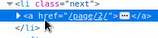
\includegraphics[width=\width\textwidth]{./figs/20220606191904.png}
        \end{figure}
        \begin{itemize}
            \item Notice the class is 'next', and the inner html is always a link to the next page.
        \end{itemize}
    
    \item Now we can get all the information distributed in multiple pages:
        \begin{minted}[autogobble]{py}
            import requests
            from bs4 import BeautifulSoup

            page = 1
            next_button = True
            while next_button:
                website = requests.get(f'http://quotes.toscrape.com/page/{page}')
                soup = BeautifulSoup(website.text, 'html.parser')
                next_button = soup.select_one('.next > a') # gets the next element and the 'a' tag
                quotes = soup.select('.quote')
                for quote in quotes:
                    text = quote.select_one('.text')
                    author = quote.select_one('.author')
                    tags = quote.select('.tag')
                print(f'Scrapping page={page}')
                page += 1

            # Scrapping page=1
            # Scrapping page=2
            # Scrapping page=3
            # Scrapping page=4
            # Scrapping page=5
            # Scrapping page=6
            # Scrapping page=7
            # Scrapping page=8
            # Scrapping page=9
            # Scrapping page=10
        \end{minted}
\end{itemize}